\documentclass{article}
\usepackage[utf8]{inputenc}

\title{100 Ideias}
%\numberofauthors{4} %  in this sample file, there are a *total*
% of EIGHT authors. SIX appear on the 'first-page' (for formatting
% reasons) and the remaining two appear in the \additionalauthors section.
%
\author{
% You can go ahead and credit any number of authors here,
% e.g. one 'row of three' or two rows (consisting of one row of three
% and a second row of one, two or three).
%
% The command \alignauthor (no curly braces needed) should
% precede each author name, affiliation/snail-mail address and
% e-mail address. Additionally, tag each line of
% affiliation/address with \affaddr, and tag the
% e-mail address with \email.
%
% 1st. author
\alignauthor
André Carvalho\\
       \affaddr{FCUP - DCC}\\
       \affaddr{Motivation Coach}\\
       \affaddr{Documenter}\\
\and
% 2nd. author
\alignauthor
André Fonseca\\
       \affaddr{FCUP - DCC}\\
       \affaddr{Task Master}\\
       \affaddr{Developer}\\
\and
% 3rd. author
\alignauthor Bruno Cabral\\
       \affaddr{FCUP - DCC}\\
       \affaddr{Resources Support}\\
       \affaddr{Researcher}\\
\and  % use '\and' if you need 'another row' of author names
% 4th. author
\alignauthor Tiago Castanheira\\
       \affaddr{FCUP - DCC}\\
       \affaddr{Mediator}\\
       \affaddr{Architect}\\
}




\date{April}

\usepackage{natbib}
\usepackage{graphicx}

\begin{document}
%\keywords{Helping\\ Caring \\ Integration}
\maketitle
\begin{abstract}
    Este relatorio olha para o trabalho que temos vindo a realizar durante o semestre. O objectivo deste  trabalho é ajudar os refugiados possibilitando uma plataforma web que os ajude a decidir sobre qual distrito do Pais no qual querem viver.Observamos que muitas destas pessoas não conhecem as culturas para a qual vão ser inseridas, e por esta razão decidimos facilitar a integração dos proprios na comunidade onde vão ser colocados.\\Esperamos que a nossa contribuição ajude os refugiados a perceber melhor e a facilitar a sua integração na comunidade portuguesa e que permitirá uma melhor consideração individual sobre estes individuos.
    
    
\end{abstract}
\section{Introdução}

%% The ``\copyrightspace'' command must be the first command after the
%% start of the first section of the body of your paper. It ensures the
%% copyright space is left at the bottom of the first column on the first
%% page of your paper.

%% \copyrightspace

    Está em curso a maior crise de refugiados desde a IIº Guerra, situação de uma enorme complexidade, para a qual não existe uma resposta simples, nem uma solução isenta de riscos/efeitos perversos.\\Portugal está por enquanto afastado do centro do problema, podendo ter a tentação de o “ignorar“. Deve ser, no entanto, solidário com os restantes países europeus na gestão desta crise humanitária.

\begin{itemize}
    \item Sensibilização e integração: Assim perante este contexto, esperamos que com a criação deste projecto consigamos sensibilizar Portugal para as questões dos direitos de refugiados e ao mesmo tempo ajudar estes na sua integração na comunidade Portuguesa com o envolvimento das instituiçoes locais.
    \item Plataforma de apoio: Dado esta situação esta a ser desenvolvido uma plataforma que promove o apoio aos refugiados na sociadade Portugesa, acolhimento e integração tendo em vista a autonomia e integração dos adultos no mercado de trabalho e das crianças na escola.A plataforma contem também informação cultural e social de cada distrito do pais. 
    \item Missão: Há a noção da urgência da ação humanitária, que pede uma resposta imediata de acolhimento, sem ignorar as intervenções com impacto a médio-longo prazo, como a estabilização política, económica e social das zonas de crise.\\Coloca-se o desafio de uma resposta  solidária e eficaz que evite os egoísmos nacionais, que não aumente a xenofobia e que seja útil.\\Existem instituições da sociedade civil com vontade, disponibilidade e experiência no acolhimento de refugiados que, através de uma plataforma web e através de um modelo colaborativo e articulado, poderiam dar um contributo para este desafio, em complementaridade com a ação do Estado Portugues. 


\end{itemize}

\section{}



\begin{figure}[h!]
\centering
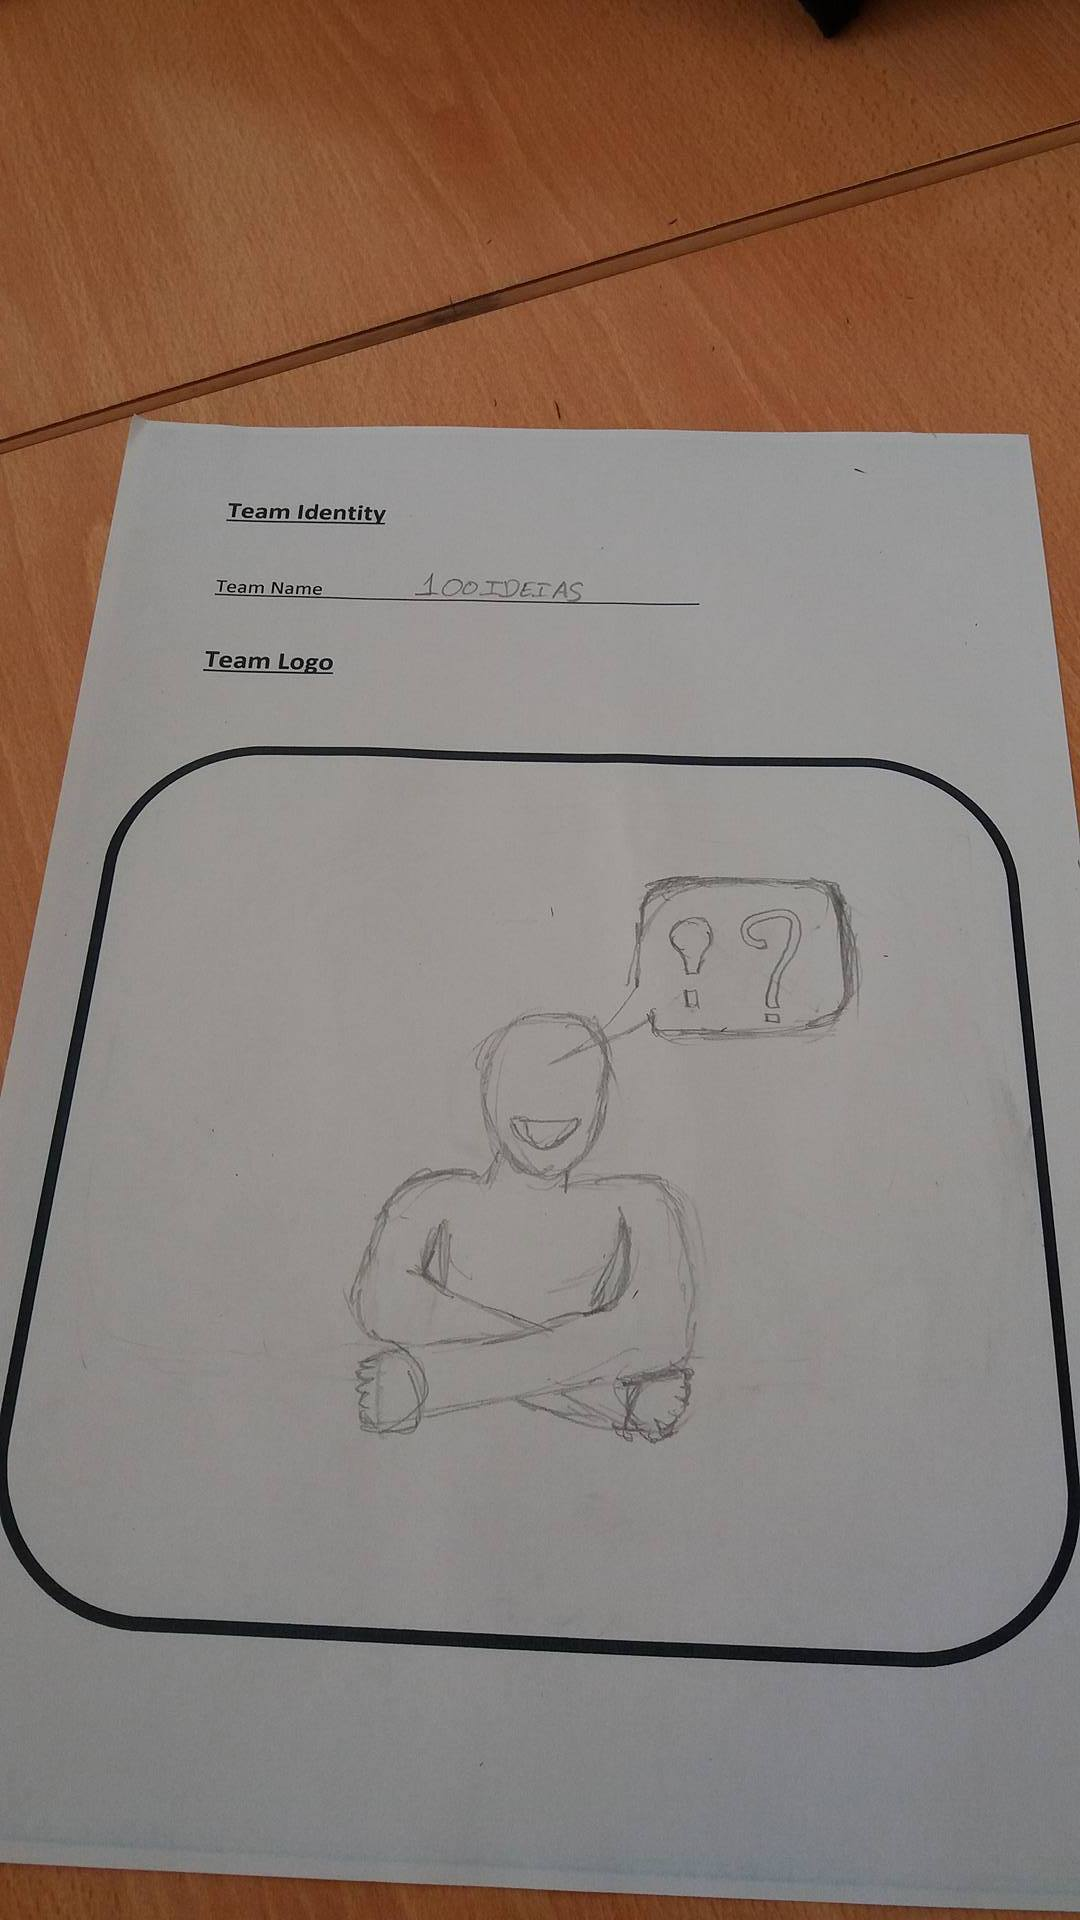
\includegraphics[scale=1.7]{logo.jpg}
\caption{The Universe}
\label{fig:univerise}
\end{figure}

\section{Conclusion}
``I always thought something was fundamentally wrong with the universe'' \citep{adams1995hitchhiker}

\bibliographystyle{plain}
\bibliography{references}
\end{document}
